\documentclass[10pt,a4paper,final]{report}
\usepackage[utf8]{inputenc}
\usepackage[english]{babel}
\usepackage{amsmath}
\usepackage{mathtools}
\usepackage{amsfonts}
\usepackage{amssymb}
\usepackage{indentfirst}
\usepackage{comment}
\usepackage{booktabs} % Allows the use of \toprule, \midrule and \bottomrule in tables

%\usepackage{graphics} % for pdf, bitmapped graphics files
\usepackage{graphicx}
\usepackage{epstopdf}
\usepackage{amsmath} % assumes amsmath package installed
\usepackage{amssymb}  % assumes amsmath package installed

\usepackage{algorithm,algorithmicx,algpseudocode}
\usepackage{amssymb}
\usepackage{subfigure}
\usepackage{comment}
\usepackage{mcode}
\usepackage{hyperref} 
\usepackage{enumitem}

\usepackage{algorithm}


\usepackage{algorithm,algorithmicx,algpseudocode}


\graphicspath{{Images/}}




\begin{document}

\title{\LARGE \bf
 Generation Evolution
}


\author{Luiz Pires\footnote{University of Porto, Portugal.} and Hugo Oliveira\footnote{University of Porto, Portugal.}}
\maketitle

\section{Introduction}
The ecosystem is represented by an $N*M$ matrix were each cell can be occupied by an object. The initial conditions (objects positions) are placed in the matrix cells and according to following rules and parameters the algorithm simulates the ecosystem evolution until an pre-determined generation number is reached.
Two implementations were made, one sequential other parallel that makes use of threads.
The following sections describes the rules in detail, the algorithm and the data structures used and implementation aspects summarizing with an performance analysis and conclusions. 



\section{Game Rules}
 The ecosystems if formed by the objects, rocks, rabbits and foxes. The world is represented by an matrix $N*M$ each one can be occupied by one of many of the objects. The simulation iterates successively following the rules until the number of generations is reached. The rules can be summarized for each generation per object as:
 
\begin{itemize}
\item ROCKS
	\begin{itemize}
 	\item The ROCKS are initially defined and during the iterations they remain in the same position.
	\end{itemize}
\item RABBITS
	\begin{itemize}
	\item The RABBITS try to move to adjacent free spaces. If free space exists, they choose according to an predefined criteria, otherwise they remain in the same place.
	\item The RABBITS can move vertical and horizontal only.
	\item The RABBITS can procreate when they pass the \textbf{GER\_PROC\_RABBITS} criteria since they are born or from last procreation. After reaching the procreation age, when an RABBIT makes an move it leaves an new RABBIT with 0 age and its procreation age returns to 0.
	\end{itemize}	
\item FOXES
	\begin{itemize}
	\item On each generation, the FOXES try to eat RABBITS by moving into adjacent cells that are occupied by RABBITS. If several adjacent cells are occupied by RABBITS, the chose one according to an predefined criteria. If no RABBIT occupies any of the adjacent cell, the move tho the free adjacent cell using the same criteria used for free cells. If no adjacent cell is occupied with RABBITS or free, they remain in the same cell.
	\item The FOXES can move horizontal and vertical only
	\item The FOXES can procreate always the pass \textbf{GER\_PROC\_FOXES} since they born or since last procreation. After reaching procreation age, when an FOX move to new cell, it leaves a new FOX with age 0 and its procrastination age return to 0.
	\item The FOXES die if they don't get feed during \textbf{GER\_ALIM\_FOXES} since they are born or they eat an RABBIT for the last time. FOXES only eat RABBITS.
	\end{itemize}
\end{itemize}
\bigskip
When one adjacent position is selected, the following rules must be considered:

\begin{itemize}
\item Numerate from 0 and following the clock pointers the position P that an RABBIT or FOXES can move: NORTH, EAST, SOUTH, WEST.
\item G being the actual generation and (X,Y) the current FOX or RABBIT coordinates, then the new space to consider is determined by (G + X + Y) mod P considering that for the initial generation is the matrix origin. 
\end{itemize}
When an space is occupied simultaneously by to animals, the conflict resolution follows the following rules

\begin{itemize}
\item When 2 or more RABBITS move to the same free cell, the older RABBIT remains and while the others disappear.
\item When 2 or more FOXES move to eat the same RABBIT, the older FOX remains while the others disappear.
\item When 2 or more FOXES move to the same free cell, the hungriest FOX (value closer to \textbf{GER\_FEED\_FOXES}) remains.
\end{itemize}


\section{System Architecture}
The system in composes by different blocks and structures in three implementations:
\begin{itemize}
\item Sequential Algorithm
\item Parallel Algorithm slicing the world in lines chunks.
\item Parallel Algorithm  with objects division (Fine Granulation)
\end{itemize}

\subsection{Main Structures and Methods}
It was created an object type that contains the type of object FOX or RABBIT and also its current position, last time has eat and auxiliary flags:\\

\textbf{Object Structure}
\begin{itemize}
\item tipo\_objeto tipo: Type of object.
\item x: Line position.
\item y: Column position.
\item gen: Generation of the object.
\item proc: Flag to procreate.
\item comida: Current food state.
\end{itemize}

\bigskip

To keep the state of the system an struct eco was created. It contains the world settings and the ecosystem matrix that contains pointers to the objects that relies in ecosystem. Each eco struct contains among other information the following attributes:\\

\textbf{Eco Structure}
\begin{itemize}
\item executeCicloThreadCoelhos: Main loop to iterate the generations of RABBITS.
\item executeCicloThreadRaposas: Main loop to iterate the generation of FOXES.
\item processaObjeto: Process the object according to the type.
\item verificaPossibilidades: Check the neighbor space of the object to find empty space or objects.
\item moveObjeto:  Moves the object to its new position according to the rules.
\item adicionaObjetoLimpezaPos: Add object so that the current pointer of the equivalent position in the matrix can be cleared and the next position can be set
\item adicionaObjetoLimpezaMem: Add object to the garbage collector to be later cleaned from memory.
\item resolveConflito: Solves the RABBITS and FOXES conflicts according to the rules.

\end{itemize}
\bigskip

The algorithm make used of the following methods/functions of order to accomplish the task of simulating the environment according to the defined rules. These methods are quickly described as:
\textbf{Main Methods}
\begin{itemize}
\item executeCicloThreadCoelhos: Main loop to iterate the generations of RABBITS.
\item executeCicloThreadRaposas: Main loop to iterate the generation of FOXES.
\item processaObjeto: Process the object according to the type.
\item verificaPossibilidades: Check the neighbor space of the object to find empty space or objects.
\item moveObjeto:  Moves the object to its new position according to the rules.
\item adicionaObjetoLimpezaMem: Add object to the garbage collector to be later cleaned from memory.
\item resolveConflito: Solves the RABBITS and FOXES conflicts according to the rules.


\end{itemize}



  
\section{Implementation}
An initial implementation make use of full sequential method. The~\ref{seqVersion} algorithm summarizes the main steps carry out.


\subsection{Sequential Version}
\begin{lstlisting}[language=c,frame=single,basicstyle=\footnotesize,caption={Sequential Version.},label=seqVersion]
- From  0 to N generation:
  - For all matrix positions:
    Processa Coelho // Simulates Rabbit
  	Limpa lista de posicoes
  	Processa Raposa // Simulates Foxes
    Limpa lista de posicoes
    Efectua Limpeza de memoria
    
\end{lstlisting}

\begin{table}[H]
\begin{center}
    \begin{tabular}{ | l | c | c |}
      \hline
      \textbf{Trial} & \textbf{Size} & \textbf{Time (s)} \\ \hline
	  1 (sequential) & 200x200 & 39.03s  \\ \hline      
      1 (sequential) & 100X100 & 3.29s  \\ \hline
	  1 (sequential) & 20x20 & 0.01s  \\ \hline
	  1 (sequential) & 10x10 & 0.00s  \\ \hline
	  
  \end{tabular}
  \caption{Sequential results}
  \label{tbl:resultados1}
\end{center}
\end{table}

Analysis the callgrind tree graph for the sequential version~\ref{fig_call_sp} the vast majority of the time was spent moving the object and checking for possibilities.

\begin{figure}[H]
      \centering
      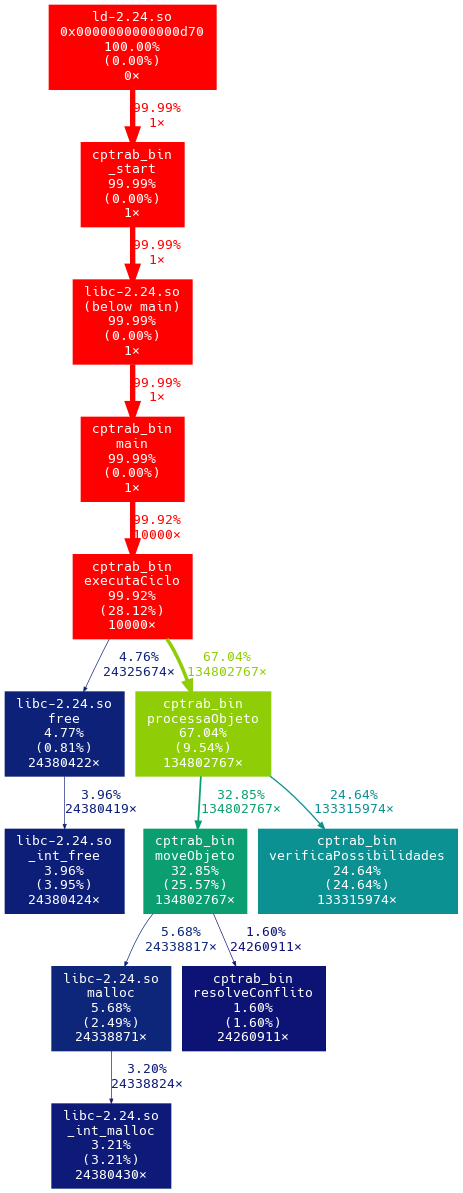
\includegraphics[height=14cm,width=10cm]{grafico_sp_200x200.png}
	        
      \caption{Callgrind tree for 200x200 input.}
      \label{fig_call_sp}
\end{figure}



\subsection{Parallel Version}

The parallel is decomposed into two main versions. The first one implements a fine to medium or large granularity by making use of a pool of threads in order to reduce its allocation and removal. Each thread is responsible for a sub area.  The second parallel version implements an fine granularity using an different approach were each thread is allocated to each object of the ecosystem instead of sub-region area. In both cases the use of a pool of threads is made in order to reduce the costs on initializing and destroying threads.


\subsubsection{Medium to Large Granularity (Sub matrix area decomposition)}
We consider a large granularity when the ratio between the number of cell that each thread is responsible is very large when compared to the number of available working threads.
In this configuration the main objective is to reduce the use of the mutex to the minimal. As described, the threads division follow the matrix line division of the ecosystem. The mutex is only used on the frontiers lines where thread conflicts may arise, minimizing the lock time on each thread. The area decomposition by threads makes use of logic conditions to allocate working threads to their respective areas combined with mutex to handle frontier situations. The Figure~\ref{fig_submatrix} presents a possible matrix area decomposition per thread. 

\begin{figure}[H]
      \centering
      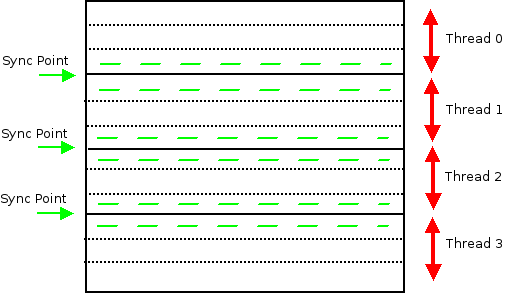
\includegraphics[height=6cm,width=10cm]{matrixDiv.png}
	        
      \caption{Matrix Sub Division by Threads.}
      \label{fig_submatrix}
\end{figure}

Initially, the each ecosystem sub-matrix is assigned to each of the available threads in order to simulate the evolution of the objects that relies in the sub space. When the thread reaches the frontier line of each sub-division, tries to take the mutex in order to avoid conflicts with the surrounding threads that may be working in the same frontier line when searching for objects or procreating to empty space, namely the North and South orientations. The algorithm~\ref{parVersion} summarizes the main parallel implementation.

\begin{lstlisting}[language=c,basicstyle=\footnotesize,frame=single,caption={Parallel Version.},label=parVersion]
- Loop:
  - 
  - While all the threads are not completed:
  - Assign threads pool to Simulate Rabbits
  - Wait for Rabbits threads to finish
  - Position cleaning (Updates matrix current and next pointers)
  - Assign threads to Simulate Foxes
  - Position cleaning (Updates matrix current and next pointers)
  - Memory Cleaning
\end{lstlisting}

The method preparaThreads() is responsible to split the work among the available threads and executaCiclo() of using the pool of threads to assign the threads to execute their partial work. The order of the main events such as simulating Rabbits, Foxes and Cleaning must be keep in the original order to produce the same results as the sequential version. Each of these sub-tasks are added to the work using the thpool\_add\_work function. Some more details were added such as the requer\_mutex in order to asses if the current processing line is a sub-matrix frontier that require a exclusion mechanism. Otherwise the thread continues its work normally.
The simulations were carryout using in the same dataset as the sequential version changing the number of threads available. For simplicity of analysis only the largest case 200x200 is presented for large granularity analysis.

\begin{table}[H]
  \begin{center}
    \begin{tabular}{ | l | c | c | c |}
      \hline
      \textbf{Trial} & \textbf{\textit{Threads}} & \textbf{Size} & \textbf{Time (s)}\\ \hline
      1 & 1 & 200x200 & 46.26s \\ \hline
      2 & 2 & 200x200 & 37.13s \\ \hline
      3 & 4 & 200x200 & 42.13s \\ \hline
      4 & 6 & 200x200 & 60.94s \\ \hline
      5 & 8 & 200x200 & 75.55s \\ \hline
     
  \end{tabular}
  \caption{Results using 200x200 with large granularity}
  \label{tbl:resultados2}
  \end{center}
\end{table}

In table~\ref{tbl:resultados2}, the increase of the number of processing by two lead to the reduction of the overall processing time, however the continuous increase of the number of threads maintaining the problem size lead to the degradation of the speedup due to the reduction of the granularity. A fine analysis is presented using the  callgrind hook graph, Figure~\ref{fig_call_mp1}.

\begin{figure}[H]
      \centering
      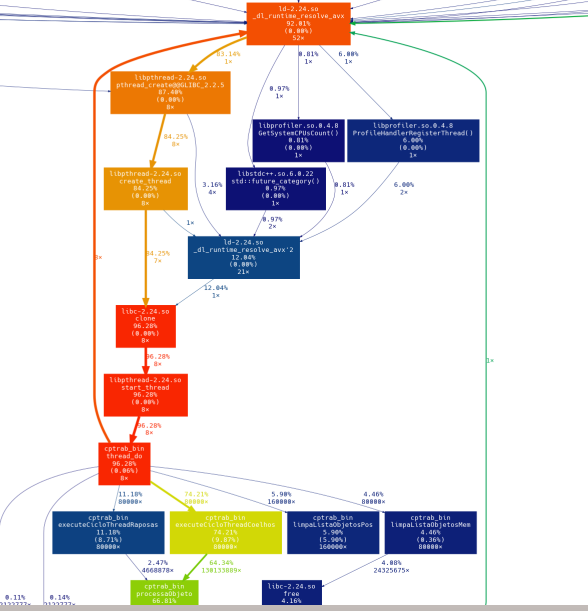
\includegraphics[height=14cm,width=10cm]{sub_grafico_mp1_8_200x200.png}
	        
      \caption{Callgrind tree for 200x200 input using 8 threads.}
      \label{fig_call_mp1}
\end{figure}

The overall performance was affected by the inclusion of code to create the threads and assign work to the threads as expected. In more detail, we can observe that when using 2 threads the mutex was never used, while the version with 8 threads makes use of the mutex, Figures~\ref{fig_lock_2}~\ref{fig_lock_8}.

\begin{figure}[H]
      \centering
      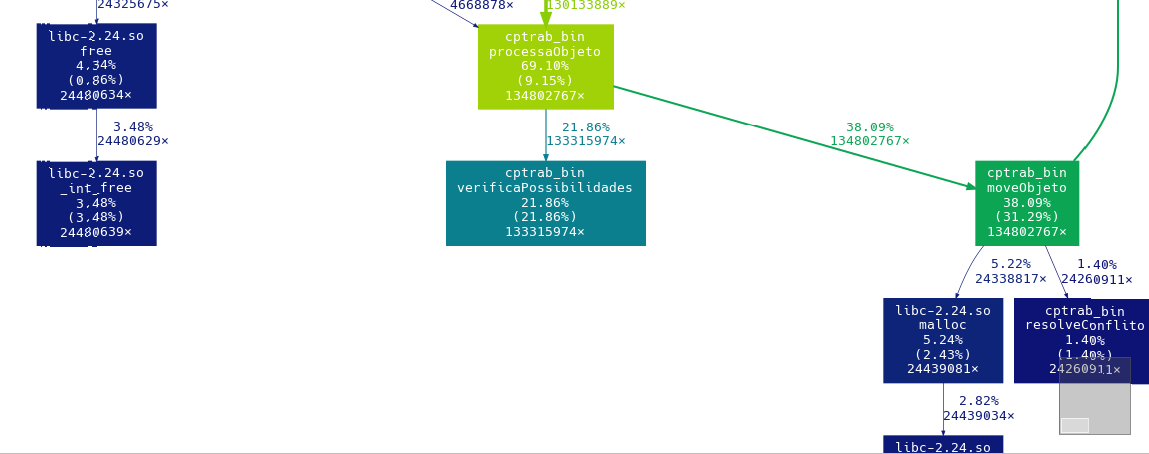
\includegraphics[height=8cm,width=12cm]{sub_grafico_mp1_2_200x200_Lock.png}
	        
      \caption{Locking time using 2 Threads.}
      \label{fig_lock_2}
\end{figure}

\begin{figure}[H]
      \centering
      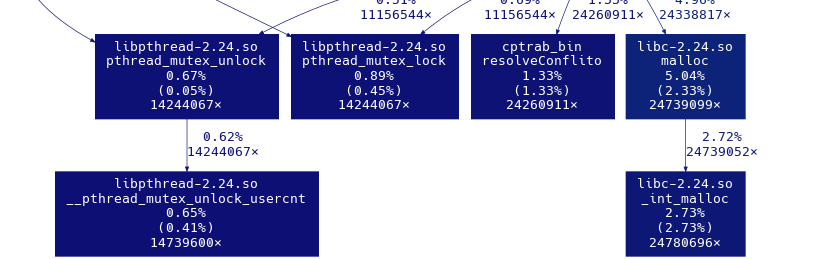
\includegraphics[height=8cm,width=12cm]{sub_grafico_mp1_8_200x200_Lock.png}
	        
      \caption{Locking time using 8 Threads.}
      \label{fig_lock_8}
\end{figure}


The use of the mutex is due to the fact that the assigned area for each thread is smaller, and according to the ecosystem density some threads may evolve faster than others, resulting in race conditions in the frontiers. In this graph is visible the impact of the granularity of the work. Some threads can finish earlier while others take more time, but at the end all threads must complete their work in order to proceed to the next step of the cycle (synchronization point) by using the thpool\_wait().


\subsubsection{Fine Granularity (Sub matrix area decomposition)}

We consider a fine granularity when the ratio between the number of cells of each thread is responsible is small when compared to the number of available threads. In this analysis we decomposing the area  by lines using a large number of threads operating in a small area for each thread. The table~\ref{tbl:resultados3} present the results using a small world size while increasing the number of threads. 


\begin{table}[H]
  \begin{center}
     \begin{tabular}{ | l | c | c | c |}
      \hline
      \textbf{Trial} & \textbf{\textit{Threads}} & \textbf{Size} & \textbf{Time (s)}\\ \hline
      1 & 1 & 20x20 & 0.42s \\ \hline
      2 & 2 & 20x20 & 0.50s \\ \hline
      3 & 4 & 20x20 & 0.54s  \\ \hline
      4 & 6 & 20x20 & 1.38s \\ \hline
      5 & 8 & 20x20 & 1.48s \\ \hline
      
  \end{tabular}
  \caption{Result using 20x20 with fine granularity}
  \label{tbl:resultados3}
  \end{center}
\end{table}

The table demonstrates clearly the impact of the increasing number of threads while the area to be processed decreases. Analyzing in more fine detail, Figures~\ref{fig_lock_88} we can observe that for 2 and 8 threads exists a increase condition signals to test the mutex.



\begin{figure}[H]
    	  \subfigure[Locking time using 2 Threads.]{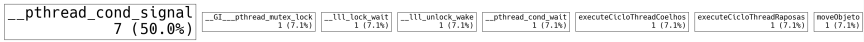
\includegraphics[width=0.49\textwidth]{grafico_prof_mp1_2_20x20.png}}
    \subfigure[Locking time using 8 Threads.]{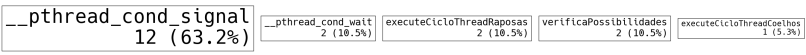
\includegraphics[width=0.49\textwidth]{grafico_prof_mp1_8_20x20.png}}
      \label{fig_lock_88}
\end{figure}



\subsubsection{Fine Granularity (Object level)}
The second parallel version assigns threads to each object sequentially instead of area decomposition.
The objective was to reduce the thread activity, being each thread responsible by moving one single object at time. This leads to the increase of the mutex use, while the active waiting in the synchronization point is very low (fewer conflicts and computational time very low). Basically the function executaCiclo(), were each object was moved directly in the main process, now each thread moves a single object and when it finish executes the next object that is waiting to be processed.
The table~\ref{tbl:resultados4} presents the attained results for the performed simulation.

\begin{table}[H]
  \begin{center}
     \begin{tabular}{ | l | c | c | c |}
      \hline
      \textbf{Trial} & \textbf{\textit{Threads}} & \textbf{Size} & \textbf{Time (s)}\\ \hline
      1 & 1 & 200x200 & 187.95s \\ \hline
      2 & 2 & 200x200 & 172.45s \\ \hline
      3 & 4 & 200x200 & 381.12s  \\ \hline
      4 & 6 & 200x200 & 1122.24s \\ \hline
      5 & 8 & 200x200 & 2134.24s \\ \hline
      
  \end{tabular}
  \caption{Result using 200x200 with ultra fine granularity}
  \label{tbl:resultados4}
  \end{center}
\end{table}

The table shows that this type of approach is totally wrong because the  granularity is extremely low. The majority of the time is spent adding and removing work from the threads, leading to a large overhead. Analyzing the callgrind tree, Figure~\ref{fig_mp2} is evident the increase of the mutex usage resulting in the decrease of the performance of the system.

\begin{figure}[H]
      \centering
      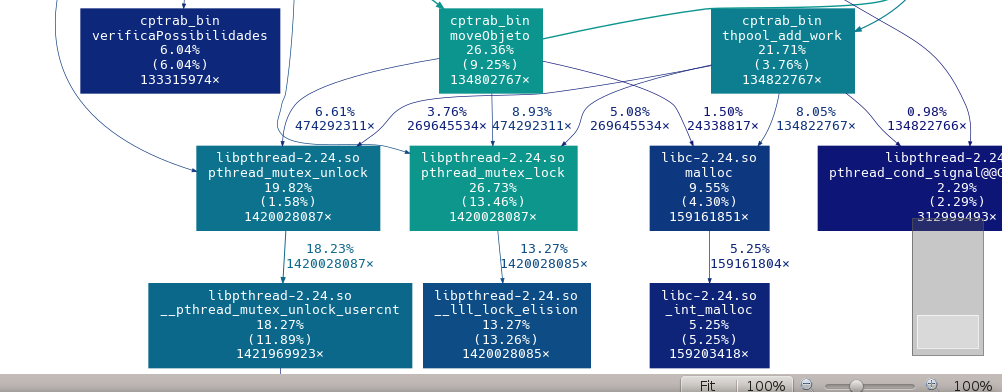
\includegraphics[height=8cm,width=12cm]{sub_grafico_mp2_8_200x200_Lock.png}
	        
      \caption{Locking time using 8 Threads.}
      \label{fig_mp2}
\end{figure}

The Figure~\ref{fig_mp2_1} shows the increase of thread assignment to works also increased.

\begin{figure}[H]
      \centering
      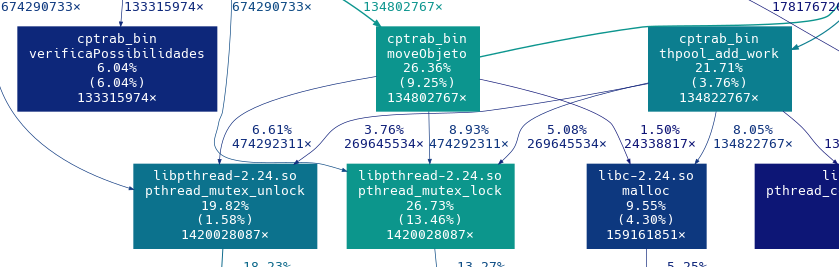
\includegraphics[height=8cm,width=12cm]{sub_grafico_mp2_8_200x201_Lock_2.png}
	        
      \caption{Locking time using 8 Threads.}
      \label{fig_mp2_1}
\end{figure}



\subsection{Analysis Medium Granularity vs Fine Granularity}
During the implementation of the first parallel version it was observed that the ratio of the number of available Threads vs number of lines affect greatly the performance of the system. This fact is due to the time spent in the system operations such adding work and removing work from the threads. If the ecosystem is very small, the system operations take the majority of the time when compared with the algorithm processing itself. Larger ratios of the world size and density vs the number of available threads increase the performance of the parallel algorithm. If the ecosystem is very small, we have the case were the threads can spent most of the time waiting to grab the mutex that is held by another threads that is currently operating on the boundary division. Also due to the fact that all threads must synchronize in predetermined points, situations were the world is extremely unbalanced, some threads may take the majority of the working time while others are just waiting in the synchronization point. On the second parallel version, no gain was achieved comparison to the sequential version. This was due to the large overhead created when assigning threads to objects itself. 


\section{Conclusions}

Analyzing the performance tables, we can verify that the performance of the algorithm is extremely affected by the parallel implementation of the first version when the ratio between ecosystem vs number of available Threads decreases.
Comparing with time taken by the sequential algorithm, points that the computations to determine if a thread has conditions to run vs the involved computation inside the critical zone are very high, degrading the performance.
The second version only further proved that the since the computational costs of the operations of moving the objects are so low, for the algorithm to scale, it needs to have the least possible amount of synchronization possible. The low granularity can make the parallel version worst than the sequential version.


\section{Final Notes}
The folder were this report is contained contains all the results simulations carryout during development and many other intermediate simulations that were not considered in the final report.

\bibliography{NONE}


\begin{thebibliography}{99}
\bibitem{pthreads} Nichols, Bradford and Buttlar, Dick and Farrell, Jacqueline, Pthreads programming: A POSIX standard for better multiprocessing, O\'Reilly Media, Inc, 1996.


\bibitem{valgrind} Seward, Julian and Nethercote, Nicholas and Weidendorfer, Josef: Valgrind 3.3-Advanced Debugging and Profiling for GNU/Linux applications, Network Theory Ltd, 2008.


\end{thebibliography}
  
\end{document}
